\documentclass[11pt, spanish]{extarticle}
\usepackage[spanish, activeacute]{babel}
\usepackage[utf8]{inputenc}
\usepackage{color}
\usepackage{graphicx}
\usepackage{parskip}
\usepackage[margin=1in]{geometry}
\usepackage{csquotes}
\parindent 0em
\setlength{\parskip}{\baselineskip}
\newcommand{\textoverline}[1]{$\overline{\mbox{#1}}$}
\newcommand{\tab}{\hspace*{2em}}
\newcommand{\HRule}{\rule{\linewidth}{0.5mm}} 


\begin{document}
\begin{titlepage}
\begin{center}

\includegraphics[scale=0.25]{USB.jpeg}~\\[1cm]

\textsc{\LARGE Universidad Simón Bolívar}\\[1.5cm]
\textsc{\Large Redes de Computadoras}\\[1.5cm]

\HRule \\[0.4cm]
{ \huge \bfseries Proyecto I: Informe\\[0.4cm] }

\HRule \\[1.5cm]
\begin{minipage}{0.4\textwidth}
\begin{flushleft} \large
\emph{Autores:}\\
Patricia Wilthew 09-10910 \\Carlos Da Silva 10-10175 \\
\end{flushleft}
\end{minipage}
\begin{minipage}{0.4\textwidth}
\begin{flushright} \large
\emph{Profesores:} \\
Ricardo Gonz'alez \\ Miguel Torrealba
\end{flushright}
\end{minipage}

\vfill
{\large \today}
\end{center}
\end{titlepage}


\tableofcontents
\newpage

\setlength\parindent{24pt}

\section{Enunciado}

Se desea que usted implemente un sistema de intercambio de mensajes cortos empleando 
para ello un conjunto de dos aplicaciones diferentes schat y cchat.

El programa schat ejercerá el rol de servidor, concentrando los mensajes que provengan de 
todos los usuarios del sistema. Cada usuario se conectará usando un programa cchat y una 
vez que esté conectado, los mensajes que escriba en su pantalla serán enviados al servidor 
schat, quien a su vez los reenviará a todos los usuarios que estén conectados a la misma sala 
en ese momento.

La sintaxis para la invocación del servidor será la siguiente: 

schat $[-p <puerto>] [-s <sala>] $

Donde: 

$<puerto>$ Es el número de puerto que el servidor utilizará para colocar un socket para 
esperar por las solicitudes de conexión que el servidor puede recibir, estas solicitudes 
podrán ser originadas por diferentes programas cchat. 

$<sala>$ Es el nombre de la sala de chat por defecto que tendrá el servidor. Si no se 
especifica ningún nombre, la sala por defecto llevará el nombre de actual los programas 
cchat que se conecten al schat se suscribirán automáticamente a esta sala al iniciar su 
conexión. 

La sintaxis para la invocación del cchat será la siguiente: 

$cchat [-h <host>] [-p <puerto>] [-n <nombre>][-a <archivo>] $
Donde: 

$<host>$ Es el nombre o dirección IP del computador donde está corriendo el programa 
schat. 

$<puerto>$ Es el número de puerto que el programa schat utilizará para recibir las 
conexiones de los diferentes programas cchat. $<nombre>$ Es el nombre de usuario que será usado en todos los mensajes que el usuario envíe al servidor y que el servidor enviará a todos los otros usuarios, incluyéndolo a 'el mismo. 

$<archivo>$ Es el nombre y dirección relativa o absoluta de un archivo de texto en el que 
en cada línea habrá un comando. Al cchat terminar de ejecuatr los comandos 
presentes en el archivo, debe permanecer a la espera de nuevos comandos por el teclado. A 
menos que, en el archivo este presente el comando $fue$
 
Un ejemplo de lo que puede tener uno de estos archivos es el siguiente: 

$sal$

$usu$

$cre$
$ gallinero$

$sal$

$men $
$hola $
$todos$
 
Los parámetros de entrada podrán venir en cualquier orden. 
 
El usuario del programa cchat podrá usar una serie de comandos que escribirá por pantalla 
y que serán enviados al programa schat. 

La lista de comandos que podrá usar es la siguiente: 

$sal$ Este comando hace que el usuario pueda ver en su pantalla una lista de las salas de 
chat que el servidor posee. 

$usu$ Este comando hace que el usuario pueda ver en su pantalla una lista actualizada de 
todos los usuarios que están suscritos en el servidor, incluyéndolo a el mismo 

$men <mensaje>$ Este comando envía el mensaje a todos los usuarios que están 
conectados al mismo servidor en la sala de chat a la que está suscrito el usuario. 

$sus <sala>$ El usuario se suscribe a la sala de chat sala. 

$des$ Este comando de-suscribe al usuario de la sala o salas a las que este suscrito 

$cre <sala>$ El usuario crea la sala en el servidor. 

$eli <sala>$ El usuario elimina la sala del servidor. 

$fue$ Este comando permite terminar la ejecución del programa de introducción de 
comandos y la ejecución del programa cchat. 

Se debe entregar un informe impreso con los siguientes contenidos:
Un diagrama de secuencia con el intercambio de mensajes que debe ocurrir entre un schat y
otros dos cchat, los dos suscritos a una misma sala de nombre actual, uno de los cuales
ejecuta los siguientes comandos:

$men$ 
$ Hola$

$usu$

$sal$

$cre$
$ nueva$

$des$

$sus $
$nueva$

$men $
$chao$
\clearpage

\section{Diagrama de secuencias}

Intercambio de mensajes que debe ocurrir entre un schat y
otros dos cchat, los dos suscritos a una misma sala de nombre actual.

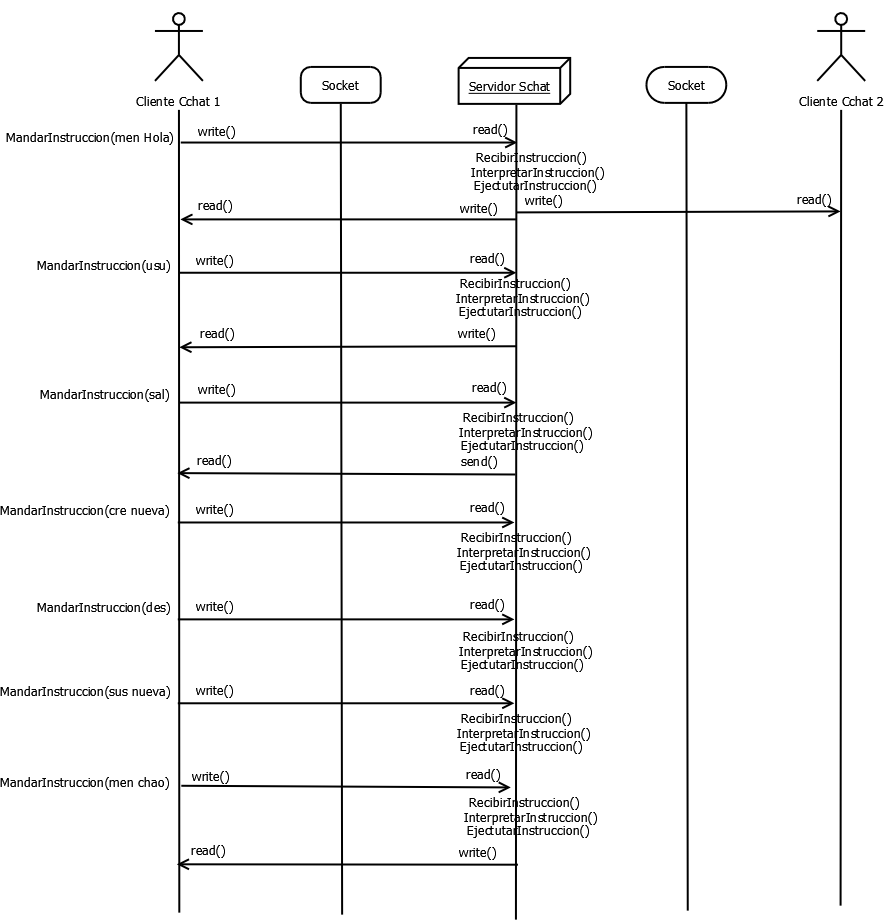
\includegraphics[width=0.85\textwidth]{C:/Users/Patricia/Dropbox/0REDES-L/SequenceDiagram.png}

\clearpage

\section{Funcionamiento}

La funcionalidad del c'odigo para schat y cchat corresponde al enunciado.

Para empezar a usarlo, primero debe hacer make y ejecutar el servidor:

schat $[-p <puerto>] [-s <sala>] $

La sala por defecto se llama Actual, en tal caso de que no se especifique.

Luego, puede conectar uno o m'as clientes ejecutando:

cchat $[-h <host>] [-p <puerto>] [-n <nombre>][-a <archivo>] $


El host puede ser la direcci'on IP de la m'aquina donde se ejecuta el server o su DNS.

El archivo es opcional. El puerto para cada cliente que se conecte debe ser igual al utilizado para ejecutar schat.

Una vez que el programa interpret'o y ejecut'o todos los comandos del archivo, puede escribir m'as comandos por entrada est'andar.

\clearpage

\section{Detalles sobre implementaci'on}
Las estructuras m'as importantes utilizadas fueron los hilos y los sockets.

Cuando el server comienza a funcionar, debe estar pendiente de que nuevos clientes quieran conectarse y su vez debe estar al tanto de todos los cambios hechos por cada uno de los clientes para poder hacer llegar esos cambios a los dem'as. Este problema pudo dividirse en subtareas, cada una de ellas resuelta con hilos.

La lista de usuarios con sus respectivas salas y la lista de salas disponibles en el servidor, son variables globales en el c'odigo. Luego, toda la informaci'on que se intercambia entre el servidor y los clientes se logra a trav'es de los sockets.

Para m'as informaci'on sobre la implementaci'on, se sugiere ver el c'odigo.

\clearpage

\end{document}

